\documentclass[12pt]{article}

\usepackage[english]{babel}
\usepackage[utf8]{inputenc}
\usepackage{sansmathfonts}
\usepackage[T1]{fontenc}
\renewcommand*\familydefault{\sfdefault} %% Only if the base font of the document is to be sans serif
\usepackage{multicol,lipsum}
\usepackage{amsmath,cancel}
\usepackage{amssymb,amsthm,dsfont,mathrsfs}
\usepackage[colorinlistoftodos]{todonotes}
\usepackage{geometry}
\geometry{
a4paper,
total={170mm,257mm},
left=20mm,
top=15mm,
bottom=22mm,
}
\usepackage{natbib}
\usepackage{soul}
\usepackage{setspace}
\usepackage{hyperref}
\usepackage{xcolor}
\usepackage{graphicx}
\usepackage{tikz}
\usepackage{siunitx}
\graphicspath{ {imagens/} }
\usepackage{fancyhdr}
\pagestyle{fancy}
\renewcommand{\headrulewidth}{0pt}

\color{darkgray}
\newcommand{\T}[1]{\vspace{0.4cm}\textbf{\large#1}}
\newcommand{\TW}[1]{\textbf{\large#1}}

\newcommand{\TM}[1]{\vspace{0.2cm} \textbf{#1}}

\newcommand{\M}[1]{
\vspace{-0.6cm}
\begin{flalign*}
#1&
\end{flalign*}
\vspace{-0.6cm}
}


\definecolor{bluebell}{rgb}{0.25, 0.35, 0.89} 
\definecolor{laranja}{rgb}{0.87, 0.48, 0.25} 
\definecolor{verde}{rgb}{0, 0.54, 0.44} 
\definecolor{babypink}{rgb}{1, 0.42, 0.52} 
\definecolor{rosa}{rgb}{1, 0.72, 0.77} 
\definecolor{cinza}{rgb}{0.3, 0.3, 0.3}  
\definecolor{iris}{rgb}{0.25, 0.35, 0.89}  
\definecolor{babyblue}{rgb}{0.13, 0.59, 0.95}

\setlength\columnsep{30pt}

\setlength{\parindent}{0cm}
\setlength{\fboxrule}{1.3pt}  % <-- Aumenta a espessura

\newcommand{\Formula}[1]{
\begin{center}
\color{iris}
\fcolorbox{rosa}{white}{
\(
\begin{array}{c}
#1
\end{array}
\)
}
\color{cinza}
\end{center}
}

\begin{document}
\pagenumbering{gobble}
\setstretch{1.3}


\includegraphics[width=4cm]{Logo2.png}
\begin{center}
    \textbf{\Huge \textcolor{bluebell}{Geometria Analítica}}
\end{center}

\begin{multicols}{2}

% ── PONTO NO PLANO ─────────────────────────────────────────────────────────
\TW{Ponto no Plano Cartesiano}

Todo ponto $P$ é identificado pelo par ordenado $(x, y)$: $x$ é a \textbf{abscissa}
(horizontal) e $y$ é a \textbf{ordenada} (vertical).

\TM{Distância entre dois pontos:}

\Formula{d_{AB} = \sqrt{(x_2-x_1)^2 + (y_2-y_1)^2}}

$\Delta x$ e $\Delta y$ são os catetos; $d_{AB}$ é a hipotenusa (Pitágoras).

\TM{Ponto médio:}

\Formula{M = \left(\dfrac{x_1+x_2}{2},\;\dfrac{y_1+y_2}{2}\right)}

\TM{Exemplos — $A(1,2)$ e $B(4,6)$:}

$d_{AB} = \sqrt{9+16} = \sqrt{25} = \boxed{5}$

$M = \left(\dfrac{5}{2},\; 4\right)$

\TM{$A(-3,1)$ e $B(1,-3)$:}

$d_{AB} = \sqrt{16+16} = \sqrt{32} = 4\sqrt{2} \approx 5{,}66$

% ── EQUAÇÃO DA RETA ────────────────────────────────────────────────────────
\TW{Equação da Reta}

\begin{center}
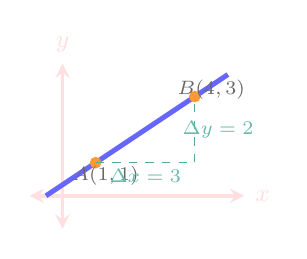
\begin{tikzpicture}[scale=0.42]
\tikzstyle{eixo}=[pink!50!white, line width=1.3pt]
\draw[eixo, stealth-stealth] (-1,0) -- (5.5,0) node[right, font=\small] {$x$};
\draw[eixo, stealth-stealth] (0,-1) -- (0,4) node[above, font=\small] {$y$};
\draw[blue!60!white, line width=1.8pt, domain=-0.5:5] plot (\x, {2/3*\x+1/3});
\filldraw[orange!80!white] (1,1) circle (4.5pt);
\filldraw[orange!80!white] (4,3) circle (4.5pt);
\node[font=\scriptsize, black!60!white] at (1.3,0.6) {$A(1,1)$};
\node[font=\scriptsize, black!60!white] at (4.5,3.2) {$B(4,3)$};
\draw[dashed, verde!70!white] (1,1) -- (4,1) -- (4,3);
\node[font=\scriptsize, verde!60!white] at (2.5,0.6) {$\Delta x=3$};
\node[font=\scriptsize, verde!60!white] at (4.7,2.0) {$\Delta y=2$};
\end{tikzpicture}
\end{center}

\TM{Forma reduzida:} $\;y = mx + b$ \hfill ($m$: inclinação; $b$: intersecção)

\TM{Forma ponto-inclinação:} $\;y - y_1 = m(x - x_1)$

\TM{Forma geral:} $\;ax + by + c = 0$

\TM{Exemplo — reta por $A(1,1)$ e $B(4,3)$:}

$m = \dfrac{3-1}{4-1} = \dfrac{2}{3}$; \quad $y - 1 = \dfrac{2}{3}(x-1)$

$\Rightarrow y = \dfrac{2}{3}x + \dfrac{1}{3}$ \quad (geral: $2x - 3y + 1 = 0$)

% ── COEFICIENTE ANGULAR ────────────────────────────────────────────────────
\TW{Coeficiente Angular}

\Formula{m = \dfrac{\Delta y}{\Delta x} = \dfrac{y_2 - y_1}{x_2 - x_1}}

\TM{Retas paralelas:} mesma inclinação, $b$ diferente.

\Formula{r_1 \parallel r_2 \;\Leftrightarrow\; m_1 = m_2}

\TM{Retas perpendiculares:} produto das inclinações é $-1$.

\Formula{r_1 \perp r_2 \;\Leftrightarrow\; m_1 \cdot m_2 = -1}

\TM{Exemplo:} reta $y = 3x - 2$ tem $m = 3$. Perpendicular: $m_\perp = -\tfrac{1}{3}$.

\fcolorbox{laranja}{white}{\parbox{0.85\linewidth}{
\small\textbf{Casos especiais:} reta horizontal: $m = 0$, equação $y = k$.
Reta vertical: $m$ indefinido, equação $x = k$.
}}

% ── POSIÇÕES RELATIVAS ─────────────────────────────────────────────────────
\TW{Posições Relativas de Duas Retas}

\begin{itemize}
\item \textbf{Paralelas distintas:} $m_1 = m_2$ e $b_1 \neq b_2$ — sem ponto comum
\item \textbf{Concorrentes:} $m_1 \neq m_2$ — um ponto de interseção
\item \textbf{Coincidentes:} $m_1 = m_2$ e $b_1 = b_2$ — infinitos pontos
\end{itemize}

\TM{Exemplo — concorrentes:}

$r_1: y = x+1$ e $r_2: y = -x+5$

$x+1 = -x+5 \;\Rightarrow\; 2x = 4 \;\Rightarrow\; x = 2,\; y = 3$

Interseção: $\boxed{(2, 3)}$

% ── DISTÂNCIA PONTO–RETA ───────────────────────────────────────────────────
\TW{Distância Ponto–Reta}

\Formula{d(P,\,r) = \dfrac{\,|ax_0 + by_0 + c|\,}{\sqrt{a^2+b^2}}}

\TM{Exemplo 1 — $P(3,-1)$ e reta $2x - y + 4 = 0$:}

$d = \dfrac{|6 + 1 + 4|}{\sqrt{5}} = \dfrac{11}{\sqrt{5}} = \dfrac{11\sqrt{5}}{5} \approx 4{,}92$

\TM{Exemplo 2 — $O(0,0)$ e reta $3x + 4y - 15 = 0$:}

$d = \dfrac{|{-15}|}{\sqrt{9+16}} = \dfrac{15}{5} = \boxed{3}$

% ── EQUAÇÃO DA CIRCUNFERÊNCIA ──────────────────────────────────────────────
\TW{Equação da Circunferência}

Centro $C(a,b)$ e raio $r$ — forma canônica:

\Formula{(x - a)^2 + (y - b)^2 = r^2}

Forma geral: $x^2 + y^2 + Dx + Ey + F = 0$.

Para converter da geral à canônica, use \textbf{completamento de quadrados}.

\begin{center}
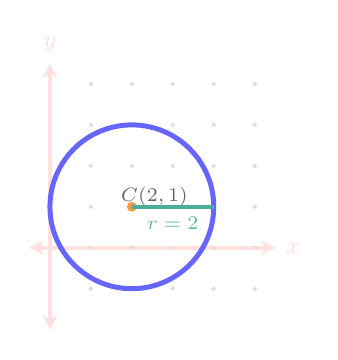
\begin{tikzpicture}[scale=0.52]
\tikzstyle{eixo}=[pink!50!white, line width=1.3pt]
\draw[eixo, stealth-stealth] (-0.5,0) -- (5.5,0) node[right, font=\small] {$x$};
\draw[eixo, stealth-stealth] (0,-2) -- (0,4.5) node[above, font=\small] {$y$};
\foreach \x in {1,2,3,4,5} \foreach \y in {-1,0,1,2,3,4}
  \filldraw[gray!25!white] (\x,\y) circle (1.2pt);
\draw[blue!60!white, line width=1.8pt] (2,1) circle (2);
\filldraw[orange!80!white] (2,1) circle (3pt);
\node[font=\scriptsize, black!60!white] at (2.55,1.25) {$C(2,1)$};
\draw[verde!70!white, line width=1.4pt] (2,1) -- (4,1);
\node[font=\scriptsize, verde!60!white] at (3.0,0.6) {$r=2$};
\end{tikzpicture}
\end{center}

\TM{Exemplo 1:} centro $C(3,-2)$, raio 4:

$(x-3)^2 + (y+2)^2 = 16$

Forma geral: $x^2 + y^2 - 6x + 4y - 3 = 0$

\TM{Exemplo 2 — identificar centro e raio:}

$x^2+y^2-4x+6y+4=0$

$(x^2-4x+4) + (y^2+6y+9) = -4+4+9$

$(x-2)^2 + (y+3)^2 = 9$

Centro $C(2,-3)$, raio $r = 3$

% ── POSIÇÃO PONTO–CIRCUNFERÊNCIA ───────────────────────────────────────────
\TW{Posição Ponto–Circunferência}

Calcule $d = d(P, C)$ e compare com $r$:

$d < r$ → interior \quad $d = r$ → na curva \quad $d > r$ → exterior

\TM{Exemplo:} $(x-2)^2 + (y-1)^2 = 9$, $C(2,1)$, $r = 3$.

$A(5,1)$: $d = \sqrt{9+0} = 3 = r$ → \textbf{na circunferência}

$B(0,0)$: $d = \sqrt{4+1} = \sqrt{5} < 3$ → \textbf{interior}

\fcolorbox{laranja}{white}{\parbox{0.85\linewidth}{
\small\textbf{Atalho:} substitua $(x_0, y_0)$ no lado esquerdo da equação canônica.
Se o resultado for $< r^2$ → interior; $= r^2$ → na curva; $> r^2$ → exterior.
}}

\end{multicols}

\lfoot{\scriptsize © Copyright, Pratique Já}
\cfoot{\large \textcolor{bluebell}{pratiqueja.com}}
\end{document}
